\documentclass[11pt]{article}
\usepackage{geometry}
\geometry{margin=1in}
\usepackage{amsmath}
\usepackage{amssymb}
\usepackage{enumitem}
\usepackage{parskip}
\usepackage{xcolor}
\usepackage{tikz}
\definecolor{benblue}{HTML}{1769AA}

\newcommand{\drawbox}[1]{%
  \par\vspace{4pt}\noindent
  \fbox{\rule{0pt}{#1}\rule{\dimexpr\linewidth-2\fboxsep-2\fboxrule}{0pt}}%
  \par\vspace{6pt}}

\newcommand{\task}[1]{\par\medskip\noindent\textbf{\color{benblue}#1}\par\nopagebreak}

\title{\vspace{-1.5cm}\textbf{Tilings}\\[-2pt]
  \large Why only three shapes fill the floor}
\author{}
\date{}

\begin{document}
\maketitle
\vspace{-1.2cm}

\noindent\textbf{The question.} A tiling covers the floor with no gaps and no
overlaps. If every tile is the \emph{same} regular polygon, which shapes can do
it? Try it first, then prove which ones must work.

\section*{Build: ring a single point}
Cut out a stack of identical regular triangles, squares, pentagons, and hexagons
(or use pattern blocks). For each shape, fit copies around one point, corner to
corner, and see whether they close up with no gap and no overlap.
\task{Which shapes closed up cleanly? Which left a gap or overlapped? Draw your
best pentagon attempt and circle the gap:}
\drawbox{4.5cm}

\section*{The key idea}
At any meeting-point, the corners crowding around it must sweep the \emph{whole}
turn: they add up to exactly $360^\circ$. So a regular shape tiles only when
copies of its corner angle total $360$, which means its corner angle must
\textbf{divide $360$ evenly}. The corner angle of a regular $n$-gon is
$\dfrac{(n-2)\cdot 180}{n}$ (you proved the $(n-2)\cdot 180$ part in Module 02).

\begin{center}
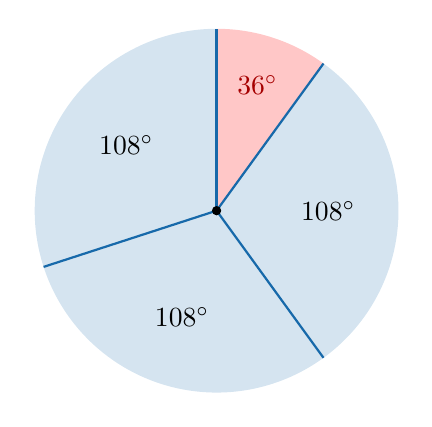
\begin{tikzpicture}[scale=1.05]
  \fill[benblue!18] (0,0) -- (90:2.2) arc (90:198:2.2) -- cycle;
  \fill[benblue!18] (0,0) -- (198:2.2) arc (198:306:2.2) -- cycle;
  \fill[benblue!18] (0,0) -- (306:2.2) arc (306:414:2.2) -- cycle;
  \fill[red!22]     (0,0) -- (54:2.2)  arc (54:90:2.2)   -- cycle;
  \draw[benblue, thick] (0,0) -- (90:2.2);
  \draw[benblue, thick] (0,0) -- (198:2.2);
  \draw[benblue, thick] (0,0) -- (306:2.2);
  \draw[benblue, thick] (0,0) -- (54:2.2);
  \node at (144:1.35) {$108^\circ$};
  \node at (252:1.35) {$108^\circ$};
  \node at (360:1.35) {$108^\circ$};
  \node[red!65!black] at (72:1.6) {$36^\circ$};
  \fill (0,0) circle (1.6pt);
\end{tikzpicture}
\end{center}
\begin{center}\small Three pentagon corners reach only $324$; a $36^\circ$ gap is
left, and a fourth pentagon will not fit.\end{center}

\section*{Fill in the table}
\task{Compute each corner angle, then decide. Use $\dfrac{(n-2)\cdot 180}{n}$.}

\begin{center}
\begin{tabular}{|l|c|c|c|c|}
\hline
shape & $n$ & corner $=\dfrac{(n-2)180}{n}$ & divides $360$? & tiles? \\[6pt] \hline
triangle & $3$ & & & \\[12pt] \hline
square   & $4$ & & & \\[12pt] \hline
pentagon & $5$ & & & \\[12pt] \hline
hexagon  & $6$ & & & \\[12pt] \hline
heptagon & $7$ & & & \\[12pt] \hline
\end{tabular}
\end{center}

\task{In one sentence: why can no regular polygon with $7$ or more sides ever
tile? (Hint: how big is its corner, and how many could meet at a point?)}
\drawbox{2.2cm}

\section*{Push further}
\begin{enumerate}[leftmargin=*]
  \item \textbf{Mix the shapes (semiregular tilings).} Allow \emph{different}
        regular polygons at a vertex, as long as the angles still total $360$ and
        every vertex looks the same. Fill in the missing angle:
        \begin{itemize}
          \item square $+$ two octagons (octagon corner $=135$):
                $90 + 135 + \underline{\hspace{1.6cm}} = 360$.
          \item triangle, hexagon, triangle, hexagon:
                $60 + 120 + 60 + \underline{\hspace{1.6cm}} = 360$.
          \item four triangles $+$ one hexagon:
                $60\times 4 + \underline{\hspace{1.6cm}} = 360$.
        \end{itemize}
        There are exactly \textbf{eight} semiregular tilings. How many can you find?
  \item \textbf{Competition gem.} Which multisets of regular-polygon corner
        angles add to exactly $360$ at a point? It is a \emph{finite} hunt (a
        big-angle polygon leaves little room). For example $3.4.4.6$ works:
        $60 + 90 + 90 + 120 = 360$. List a few more, then ask the harder
        question: which of them actually tile the whole floor? (Not all do.)
  \item \textbf{True or false?} A big enough regular polygon will eventually tile
        the plane all by itself. \hfill T \quad / \quad F
\end{enumerate}

\end{document}
